\section{What did not work: details}
\label{app:negative}
Each item states what was tried and the measured outcome. Solved counts are out of 170 development tasks, one run per arm, unless stated.

\begin{itemize}
    \item \textbf{Patch correctness is weakly readable.} A class-mean-difference direction for ``the patch being submitted is right'' reaches held-out AUC 0.61--0.62 at layers 24--28 (319 training and 152 held-out decisions per class, split by episode). A paired variant with 83 held-out decisions per class reaches 0.45--0.46. The explore direction reaches 0.77--0.83 by the same method. Writing the 0.61 direction at three strengths solved 30, 25 and 25 against 27 unedited.
    \item \textbf{Test before submitting} (wave-5 adapter) solved 17 against 30 for the adapter without the edit and 30 for its matched random control (Table~\ref{tab:schedule}, batch 4: \texttt{vfyD\_t1.0} against \texttt{w5}). A verify-more edit on the base model solved 24 against 24 unedited (control 27).
    \item \textbf{Submit sooner} (wave-5 adapter) moved behaviour as predicted (\S\ref{sec:control}). It solved 33, 26 and 27 at strengths 0.25, 0.5 and 1.0 against 36 without the edit (Table~\ref{tab:schedule}, batch 5: \texttt{sub\_t}$s$ against \texttt{w5}). Episodes that now submitted in time submitted wrong patches.
    \item \textbf{Think briefly} moved thinking tokens as predicted (\S\ref{sec:control}) and solved 28, 28 and 25 against 29 unedited.
    \item \textbf{Edits aimed at failed file edits.} We tried a gated neuron that reads ``my last edit failed'' and writes ``read the file again'', and a neuron for ``this edit will apply''. Both left the share of regenerated edits whose quoted text exists in the file at 0.65--0.70 across 240 held-out decisions (0.67 unedited; values from the project notes).
    \item \textbf{Compiling a written rule.} Two rules from \S\ref{sec:diagnosis} (``read the relevant code before your first edit''; ``quote the current file text exactly, and re-read after any edit'') solved 25, 29 and 30 (first rule, second rule, both) as prompt text against 30 unedited in one batch. As prompts, they gave no gain. We then compiled each rule into weights (Appendix~\ref{app:rule}). At 400 logged decisions, we ran the model with and without the rule in its prompt and fitted the resulting shift of the layer-18 output. On 88 held-out decisions, a rank-16 compiled edit reproduces 53\% and 41\% of the shift ($R^2$) for the two rules, and one constant neuron reproduces 25\% and 19\%. This experiment tests whether weights can reconstruct a prompt's effect on activations; it does not test whether the rule helps. Ten runs of constant-neuron rule edits in two batches solved 24--31 (mean 27.5) against 28 and 25 unedited (exact McNemar $p \geq 0.36$ for each run; two controls solved 23). An infrastructure failure cut the rank-16 batch (batch 16) short. On the 118 tasks that every arm finished, compiled edits solved 18--22 against 18 unedited and 22 for both controls.
    \item \textbf{Single-run edits in the benchmark.} GPT's re-check-after-error gate ($-2$), rank-two rotation ($-1$) and plain decision-token gate ($-1$) did not beat the unedited model of their batch (Appendix~\ref{app:calib}).
    \item \textbf{High strength.} Always-on explore-more at strength 1.0 solved 18 against 24 unedited (Table~\ref{tab:explore}).
    \item \textbf{One-shot weight deletion.} Deletion Tuning~\citep{Lu2026SurprisingEffectiveness} learns a binary mask over weights by training. We tried a one-shot variant with no optimisation step. One exact REINFORCE gradient over existing rollouts (782) ranks entries of the MLP gate projection by the first-order predicted gain from zeroing them. We restricted the candidates to 16 rows per layer in all 42 layers, so the deletion is a rank-16 LoRA update stacked on the wave-5 RL adapter. Of 1,720,320 candidate entries, 755,581 had positive predicted gain. On one batch of 64 tasks, the adapter without deletion solved 10. Deleting all chosen entries solved 8, and deleting the top 10\% solved 9. Deleting random entries in the same rows with the same counts solved 14 and 12. The gradient-chosen deletions were below both the adapter without deletion and the random deletions. This one-shot first-order variant did not help; the experiment does not test learned masks.
\end{itemize}

\begin{table}[h]
\caption{Episode cost on the 170 development tasks, batches 21--28: mean per episode for the arm and for the unedited model of the same batches; $p$ from a batch-level paired $t$ test. Claude's control is ungated and sized to a 0.125 gap.}
\label{tab:cost}
\centering
\footnotesize
\resizebox{\linewidth}{!}{\begin{tabular}{lrrrrrrr}
\toprule
 & & \multicolumn{3}{c}{Tool calls \dn} & \multicolumn{3}{c}{Seconds \dn} \\
\cmidrule(lr){3-5}\cmidrule(lr){6-8}
Arm & Batches & Arm & Unedited & $p$ & Arm & Unedited & $p$ \\
\midrule
Claude: before-first-edit gate & 6 & 12.03 & 10.61 & 0.008 & 180.6 & 170.8 & 0.055 \\
Claude: early-calls gate & 6 & 12.42 & 10.61 & 0.002 & 185.8 & 170.8 & 0.004 \\
GPT: decision-token gate + rotation & 6 & 10.88 & 10.54 & 0.33 & 168.5 & 165.0 & 0.39 \\
Gemini: explore + concise & 3 & 10.83 & 10.83 & 1.00 & 152.7 & 153.9 & 0.53 \\
Claude's random control & 4 & 11.31 & 10.55 & 0.10 & 180.6 & 179.4 & 0.76 \\
GPT's random control & 4 & 10.63 & 10.45 & 0.37 & 171.0 & 170.7 & 0.91 \\
Gemini's random control & 3 & 10.72 & 10.83 & 0.75 & 158.0 & 153.9 & 0.29 \\
\bottomrule
\end{tabular}}
\end{table}

\begin{figure}[h]
\begin{center}
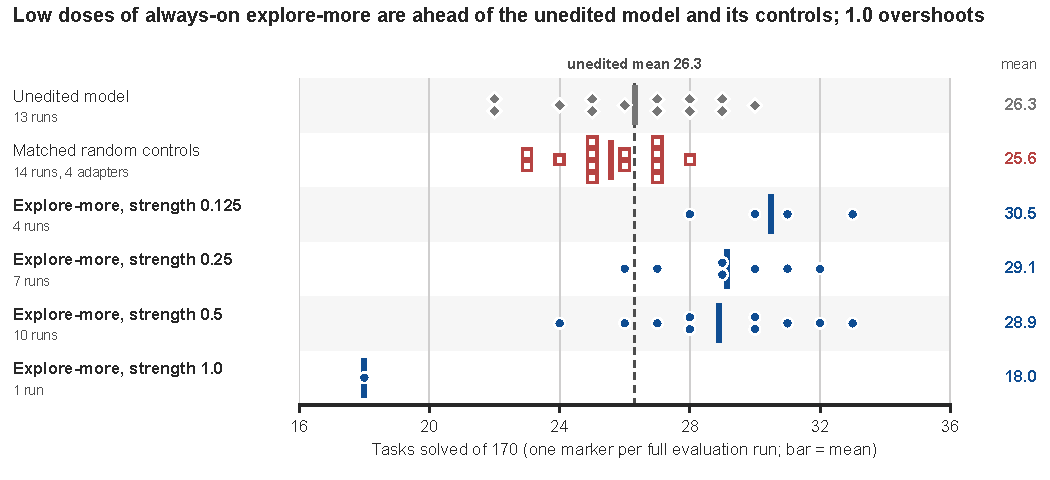
\includegraphics[width=1.0\linewidth]{figures/fig3_solve.pdf}
\end{center}
\caption{\textbf{Always-on explore-more on the development tasks.} Solved tasks of 170 per full evaluation run (one marker per run, bar = mean) for the unedited model (13 runs), matched random-direction controls (14 runs of four adapters) and the edit at four strengths. Strength 1.0 overshoots.}
\label{fig:solve}
\end{figure}
